\documentclass{article}

% Packages for various functionalities
\usepackage{lipsum} % For generating dummy text
\usepackage[margin=1in]{geometry} % Adjust margins
\usepackage{setspace} % For adjusting line spacing
\usepackage{graphicx}
\usepackage{amsmath}
\usepackage{float}
\usepackage{tikz}
\graphicspath{ {./images/} }
% Title information
\title{Neural Network Note}
\author{Muhamad Ridzuan}
\date{\today} % Use \date{} for no date or specify a date

%% tikz config
\usetikzlibrary{matrix,calc}
%isolated term
%#1 - Optional. Space between node and grouping line. Default=0
%#2 - node
%#3 - filling color
\newcommand{\implicantsol}[3][0]{
	\draw[rounded corners=3pt, fill=#3, opacity=0.3] ($(#2.north west)+(135:#1)$) rectangle ($(#2.south east)+(-45:#1)$);
}
%internal group
%#1 - Optional. Space between node and grouping line. Default=0
%#2 - top left node
%#3 - bottom right node
%#4 - filling color
\newcommand{\implicant}[4][0]{
	\draw[rounded corners=3pt, fill=#4, opacity=0.3] ($(#2.north west)+(135:#1)$) rectangle ($(#3.south east)+(-45:#1)$);
}
%group lateral borders
%#1 - Optional. Space between node and grouping line. Default=0
%#2 - top left node
%#3 - bottom right node
%#4 - filling color
\newcommand{\implicantcostats}[4][0]{
	\draw[rounded corners=3pt, fill=#4, opacity=0.3] ($(rf.east |- #2.north)+(90:#1)$)-| ($(#2.east)+(0:#1)$) |- ($(rf.east |- #3.south)+(-90:#1)$);
	\draw[rounded corners=3pt, fill=#4, opacity=0.3] ($(cf.west |- #2.north)+(90:#1)$) -| ($(#3.west)+(180:#1)$) |- ($(cf.west |- #3.south)+(-90:#1)$);
}
%group top-bottom borders
%#1 - Optional. Space between node and grouping line. Default=0
%#2 - top left node
%#3 - bottom right node
%#4 - filling color
\newcommand{\implicantdaltbaix}[4][0]{
	\draw[rounded corners=3pt, fill=#4, opacity=0.3] ($(cf.south -| #2.west)+(180:#1)$) |- ($(#2.south)+(-90:#1)$) -| ($(cf.south -| #3.east)+(0:#1)$);
	\draw[rounded corners=3pt, fill=#4, opacity=0.3] ($(rf.north -| #2.west)+(180:#1)$) |- ($(#3.north)+(90:#1)$) -| ($(rf.north -| #3.east)+(0:#1)$);
}
%group corners
%#1 - Optional. Space between node and grouping line. Default=0
%#2 - filling color
\newcommand{\implicantcantons}[2][0]{
	\draw[rounded corners=3pt, opacity=.3] ($(rf.east |- 0.south)+(-90:#1)$) -| ($(0.east |- cf.south)+(0:#1)$);
	\draw[rounded corners=3pt, opacity=.3] ($(rf.east |- 8.north)+(90:#1)$) -| ($(8.east |- rf.north)+(0:#1)$);
	\draw[rounded corners=3pt, opacity=.3] ($(cf.west |- 2.south)+(-90:#1)$) -| ($(2.west |- cf.south)+(180:#1)$);
	\draw[rounded corners=3pt, opacity=.3] ($(cf.west |- 10.north)+(90:#1)$) -| ($(10.west |- rf.north)+(180:#1)$);
	\fill[rounded corners=3pt, fill=#2, opacity=.3] ($(rf.east |- 0.south)+(-90:#1)$) -|  ($(0.east |- cf.south)+(0:#1)$) [sharp corners] ($(rf.east |- 0.south)+(-90:#1)$) |-  ($(0.east |- cf.south)+(0:#1)$) ;
	\fill[rounded corners=3pt, fill=#2, opacity=.3] ($(rf.east |- 8.north)+(90:#1)$) -| ($(8.east |- rf.north)+(0:#1)$) [sharp corners] ($(rf.east |- 8.north)+(90:#1)$) |- ($(8.east |- rf.north)+(0:#1)$) ;
	\fill[rounded corners=3pt, fill=#2, opacity=.3] ($(cf.west |- 2.south)+(-90:#1)$) -| ($(2.west |- cf.south)+(180:#1)$) [sharp corners]($(cf.west |- 2.south)+(-90:#1)$) |- ($(2.west |- cf.south)+(180:#1)$) ;
	\fill[rounded corners=3pt, fill=#2, opacity=.3] ($(cf.west |- 10.north)+(90:#1)$) -| ($(10.west |- rf.north)+(180:#1)$) [sharp corners] ($(cf.west |- 10.north)+(90:#1)$) |- ($(10.west |- rf.north)+(180:#1)$) ;
}
%Empty Karnaugh map 4x4
\newenvironment{Karnaugh}%
{
	\begin{tikzpicture}[baseline=(current bounding box.north),scale=0.8]
		\draw (0,0) grid (4,4);
		\draw (0,4) -- node [pos=0.7,above right,anchor=south west] {cd} node [pos=0.7,below left,anchor=north east] {ab} ++(135:1);
		%
		\matrix (mapa) [matrix of nodes,
		column sep={0.8cm,between origins},
		row sep={0.8cm,between origins},
		every node/.style={minimum size=0.3mm},
		anchor=8.center,
		ampersand replacement=\&] at (0.5,0.5)
		{
			\& |(c00)| 00         \& |(c01)| 01         \& |(c11)| 11         \& |(c10)| 10         \& |(cf)| \phantom{00} \\
			|(r00)| 00             \& |(0)|  \phantom{0} \& |(1)|  \phantom{0} \& |(3)|  \phantom{0} \& |(2)|  \phantom{0} \&                     \\
			|(r01)| 01             \& |(4)|  \phantom{0} \& |(5)|  \phantom{0} \& |(7)|  \phantom{0} \& |(6)|  \phantom{0} \&                     \\
			|(r11)| 11             \& |(12)| \phantom{0} \& |(13)| \phantom{0} \& |(15)| \phantom{0} \& |(14)| \phantom{0} \&                     \\
			|(r10)| 10             \& |(8)|  \phantom{0} \& |(9)|  \phantom{0} \& |(11)| \phantom{0} \& |(10)| \phantom{0} \&                     \\
			|(rf) | \phantom{00}   \&                    \&                    \&                    \&                    \&                     \\
		};
	}%
	{
	\end{tikzpicture}
}

%Empty Karnaugh map 2x4
\newenvironment{Karnaughvuit}%
{
	\begin{tikzpicture}[baseline=(current bounding box.north),scale=0.8]
		\draw (0,0) grid (4,2);
		\draw (0,2) -- node [pos=0.7,above right,anchor=south west] {bc} node [pos=0.7,below left,anchor=north east] {a} ++(135:1);
		%
		\matrix (mapa) [matrix of nodes,
		column sep={0.8cm,between origins},
		row sep={0.8cm,between origins},
		every node/.style={minimum size=0.3mm},
		anchor=4.center,
		ampersand replacement=\&] at (0.5,0.5)
		{
			\& |(c00)| 00         \& |(c01)| 01         \& |(c11)| 11         \& |(c10)| 10         \& |(cf)| \phantom{00} \\
			|(r00)| 0             \& |(0)|  \phantom{0} \& |(1)|  \phantom{0} \& |(3)|  \phantom{0} \& |(2)|  \phantom{0} \&                     \\
			|(r01)| 1             \& |(4)|  \phantom{0} \& |(5)|  \phantom{0} \& |(7)|  \phantom{0} \& |(6)|  \phantom{0} \&                     \\
			|(rf) | \phantom{00}  \&                    \&                    \&                    \&                    \&                     \\
		};
	}%
	{
	\end{tikzpicture}
}

%Empty Karnaugh map 2x2
\newenvironment{Karnaughquatre}%
{
	\begin{tikzpicture}[baseline=(current bounding box.north),scale=0.8]
		\draw (0,0) grid (2,2);
		\draw (0,2) -- node [pos=0.7,above right,anchor=south west] {b} node [pos=0.7,below left,anchor=north east] {a} ++(135:1);
		%
		\matrix (mapa) [matrix of nodes,
		column sep={0.8cm,between origins},
		row sep={0.8cm,between origins},
		every node/.style={minimum size=0.3mm},
		anchor=2.center,
		ampersand replacement=\&] at (0.5,0.5)
		{
			\& |(c00)| 0          \& |(c01)| 1  \\
			|(r00)| 0 \& |(0)|  \phantom{0} \& |(1)|  \phantom{0} \\
			|(r01)| 1 \& |(2)|  \phantom{0} \& |(3)|  \phantom{0} \\
		};
	}%
	{
	\end{tikzpicture}
}
%Defines 8 or 16 values (0,1,X)
\newcommand{\contingut}[1]{%
	\foreach \x [count=\xi from 0]  in {#1}
	\path (\xi) node {\x};
}
%Places 1 in listed positions
\newcommand{\minterms}[1]{%
	\foreach \x in {#1}
	\path (\x) node {1};
}
%Places 0 in listed positions
\newcommand{\maxterms}[1]{%
	\foreach \x in {#1}
	\path (\x) node {0};
}
%Places X in listed positions
\newcommand{\indeterminats}[1]{%
	\foreach \x in {#1}
	\path (\x) node {X};
}


\begin{document}
	\maketitle
	\section{Chapter 1}

\subsection{Donald Hebb} 
Organization of behaviour - 1949 learning mechanism:
\begin{itemize}
	\item When an axon of cell A is near enough to excite a cell B and repeatedly or persistently takes part in firing it, some growth process or metabolic change takes place in one or both cells such that A's efficiency, as on of the cells firing B, is increased.
	\item As A repeatedly excites B, its ability to excite B improves.
	\item Neuron that fire together wire together.
\end{itemize}

\subsection{Hebbian Learning}
\begin{itemize}
	\item If neuron $x$ repeatedly triggers neuron y, the synaptic knob connecting $x$ to $y$ get larger.
	\item In mathematical model:
	\[ w_{xy} = w_{xy} + \eta xy \]
	\item Weight of the connection from input neuron $x$ to output neuron $y$.
	\item This simple formula is actually the basis of many learning algorithms in machine learning.
\end{itemize}

This idea however is fundamentally unstable:
\begin{itemize}
	\item Stringer connections will enforce themselves.
	\item No notion of "competition".
	\item No \textit{reduction} in weights.
	\item Learning is unbounded.p
\end{itemize}

People came up with all kinds of modifications for it to try to make it more stable:
\begin{itemize}
	\item Allowing for weight normalization.
	\item Forgetting
\end{itemize}
This lead to the Generalized Hebbian learning, aka Sanger's rule where the contribution of input is \textit{incrementally distributed} over multiple outputs.
\[ w_{ij} = w_{ij} + \eta y_j\left( x_i -	\sum_{k=1}^{j}	w_{ik}y_k																									\right) \]

\subsection{A better model}
Frank Rosenblatt
\begin{itemize}
	\item Psychologist, Logician
	\item Inventor of the solution to everything, aka Perceptron
\end{itemize}

\paragraph{Original perceptron model}
Consider the eye structure:
\begin{itemize}
	\item Groups of sensors on retina combine into cells in association in the \textbf{projection area}.
	\item Groups of \textbf{projection area} combine into Association cells in \textbf{association area}.
	\item Signals from \textbf{association area} cells combine into response cell \textbf{R}.
	\item All connections may be excitatory or inhibitory.
\end{itemize}

Rosenblatt's perception model can then be further simplified:
\paragraph{Simplified perceptron model}

\begin{figure}[h]
	\centering
	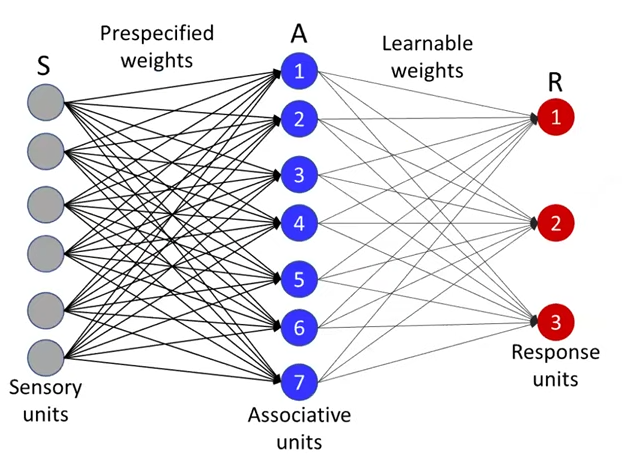
\includegraphics[scale=0.5]{simplified_perceptron_model}
\end{figure}

\begin{itemize}
	\item Association units commbine sensory input with fixed weights.
	\item Response units combine associative units with learnable weights.
\end{itemize}

Each of the units can be perceived as shown below:
\begin{figure}[h]
	\centering
	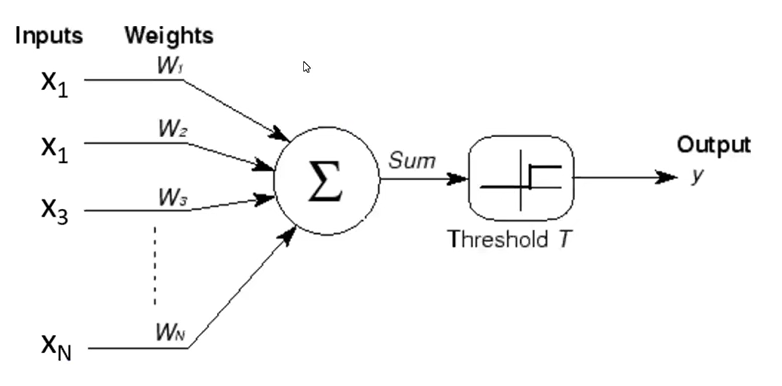
\includegraphics[scale=0.5]{perceptron_fbd}
\end{figure}

\begin{itemize}
	\item Number of inputs combine linearly.
	\item Threshold logic is applied at the output of the unit: It will only fire if the weighted sum of the input exceeds threshold.
\end{itemize}

\[ 
Y = 
\begin{cases} 
	1, & \text{if } \sum_{i}w_ix_i - T \geq 0 \\
	0, & \text{else }
\end{cases}
\]

\subsection{The Universal Model}
Originally assumed could represent any Boolean circuit and perform any logic. However this was not true and this cause the research in neural networks died down because of the overhype. However, Rosenblatt was right, he not only gave us basic model, he also gives us the learning algorithm.

\[ \mathbf{w} = \mathbf{w} + \eta (d(\mathbf{x}) - y(\mathbf{x}))\mathbf{x} \]

Sequential learning:
\begin{itemize}
	\item $d(\mathbf{x})$ is the desired output in response to input $\mathbf{x}$.
	\item $y(\mathbf{x})$ is the actual output in response to $\mathbf{x}$.
	\item Weight parameter is changed when the actual response of the neuron does not match the desired response of the neuron.
	\item If the actual response of the neuron exceeds the desired response of the neeuron, then the weight will decrease.
	\item If the actual response is lesser than the desired response, the weight will increase.
\end{itemize}

\paragraph{Single perceptron is not enough}
While this model able to mimic boolean logic such as AND, OR and NOT, it is not capable to mimic XOR gate. This imply that individual elements are weak computational elements and networked elements are required. However, with multilayered perceptron, XOR gate can be constructed:
\begin{itemize}
	\item Start with two inputs, A and B.
	\item Use AND gate to compute A and NOT B.
	\item Use another AND gate to compute NOT A AND B.
	\item Use an OR gate to combine the outputs of thee two AND gate.
\end{itemize}

This would lead to construction of perception network to represent a much more generic model:
\begin{itemize}
	\item Perceptrons can be multi-layered.
	\item Can compose arbitrarily complicated boolean functions.
	\item In cognitive terms, it should be capable to compute arbitrary boolean functions over sensory input.
\end{itemize}

\subsection{Difference between brain and neural networks}
\begin{itemize}
	\item Brains have real inputs.
	\item We are capable to make non-Boolean inferences and prediction.
\end{itemize}

\begin{figure}[h]
	\centering
	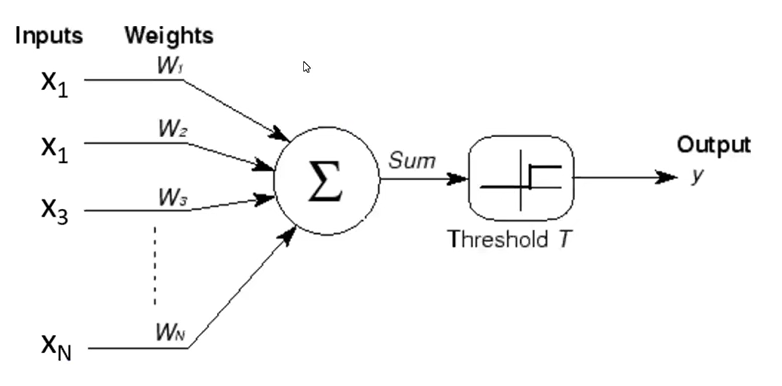
\includegraphics[scale=0.5]{perceptron_fbd}
\end{figure}

\noindent We can however try to implement \textbf{real inputs} on the perceptron model:
\begin{itemize}
	\item $x_1,x_2,...,x_N$ are real-valued.
	\item $w_1,w_2,...,w_N$ are real-valued.
	\item Unit is only fired if weighted sum of input matches or exceeds the threshold values $T$.
\end{itemize}

\begin{equation}
Y = 
\begin{cases} 
	1, & \text{if } \sum_{i}w_ix_i - T \geq 0 \\
	0, & \text{else }
\end{cases}
\end{equation}

\hfill\break
This create a boundary condition such that $\sum w_ix_i = T$ where every sum of inputs that's greater than $T$ will fire and everything that is less than $T$ would not fire.

\hfill\break
That being said, this provides an alternative view:
\begin{itemize}
	\item The neuron has a threshold \textbf{activation function} $\theta (z)$ operates on the weighted sum of inputs plus a bias. (Affine function of the inputs).
	\item The boundary $b$, is the value such that the affine term is equal to zero.
	\item Linear function is an affine function that passed through origin.
	\item $\theta (z)$ outputs a $1$ if $z$ is non-negative $0$ otherwise.
	\item Unit fires if weighted input matches or exceed threshold.
\end{itemize}
\[ 
y = \theta \left( \sum_{i}w_ix_i + b 																								\right)
\]

\[ 
\theta(z) = 
\begin{cases} 
	1, & \text{if } z \geq 0 \\
	0, & \text{else }
\end{cases}
\]

\hfill\break
On real numbers, this equation produce a hyperplane such with line separation of $w_1x_1 + w_2x_2 + ... + w_nx_n = T$ where one side of the plane is $1$ and the other side of the plane is $0$. This would means that a perceptron that operates on real-valued vectors is a type of linear classifier.

\begin{figure}[H]
	\centering
	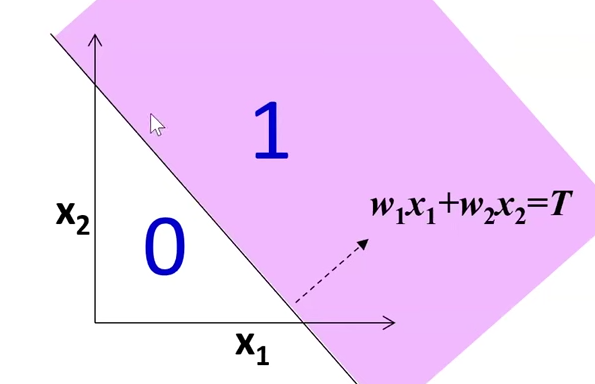
\includegraphics[scale=0.5]{hyperplane}
\end{figure}

\hfill\break
Similarly, for two-dimensional inputs, if we ever to plot the function, the function is going to looks like a step function. On one side, the output is $1$ and on the other side, the output is $0$.

\begin{figure}[H]
	\centering
	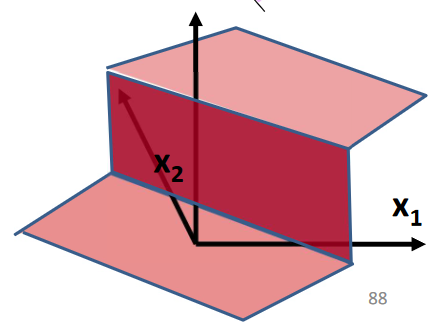
\includegraphics[scale=0.5]{2d_hyperplane}
\end{figure}

\hfill\break
Once we can see how the perceptron model works, we can finally see how it performs Boolean's functions.

\begin{figure}[H]
	\centering
	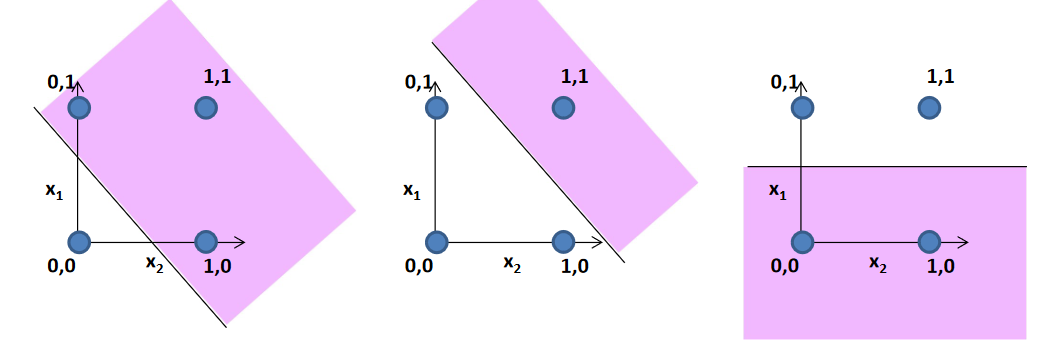
\includegraphics[scale=0.5]{1_boolean}
\end{figure}

\hfill\break
That being said, Boolean's perceptron is also linear classifiers:
\begin{itemize}
	\item Purple regions have output of $1$ in the figures.
	\item The left figure showcase OR-function.
	\item The middle figure showcase AND-function.
	\item The right figure showcase NOT-function.
	\item This is also the reason why a simple perceptron model is not enough to compose XOR-function.
\end{itemize}

\hfill\break
We can however, compose complicated decision boundaries by combining multiple linear perceptron by building a network of units with single output that firees if the input is in the desired regions. For example, we can use 5 perceptron model to compose 5 boundary condition of a pentagon. For each perceptron, the network will fire if the input is in the yellow area.

\begin{figure}[H]
	\centering
	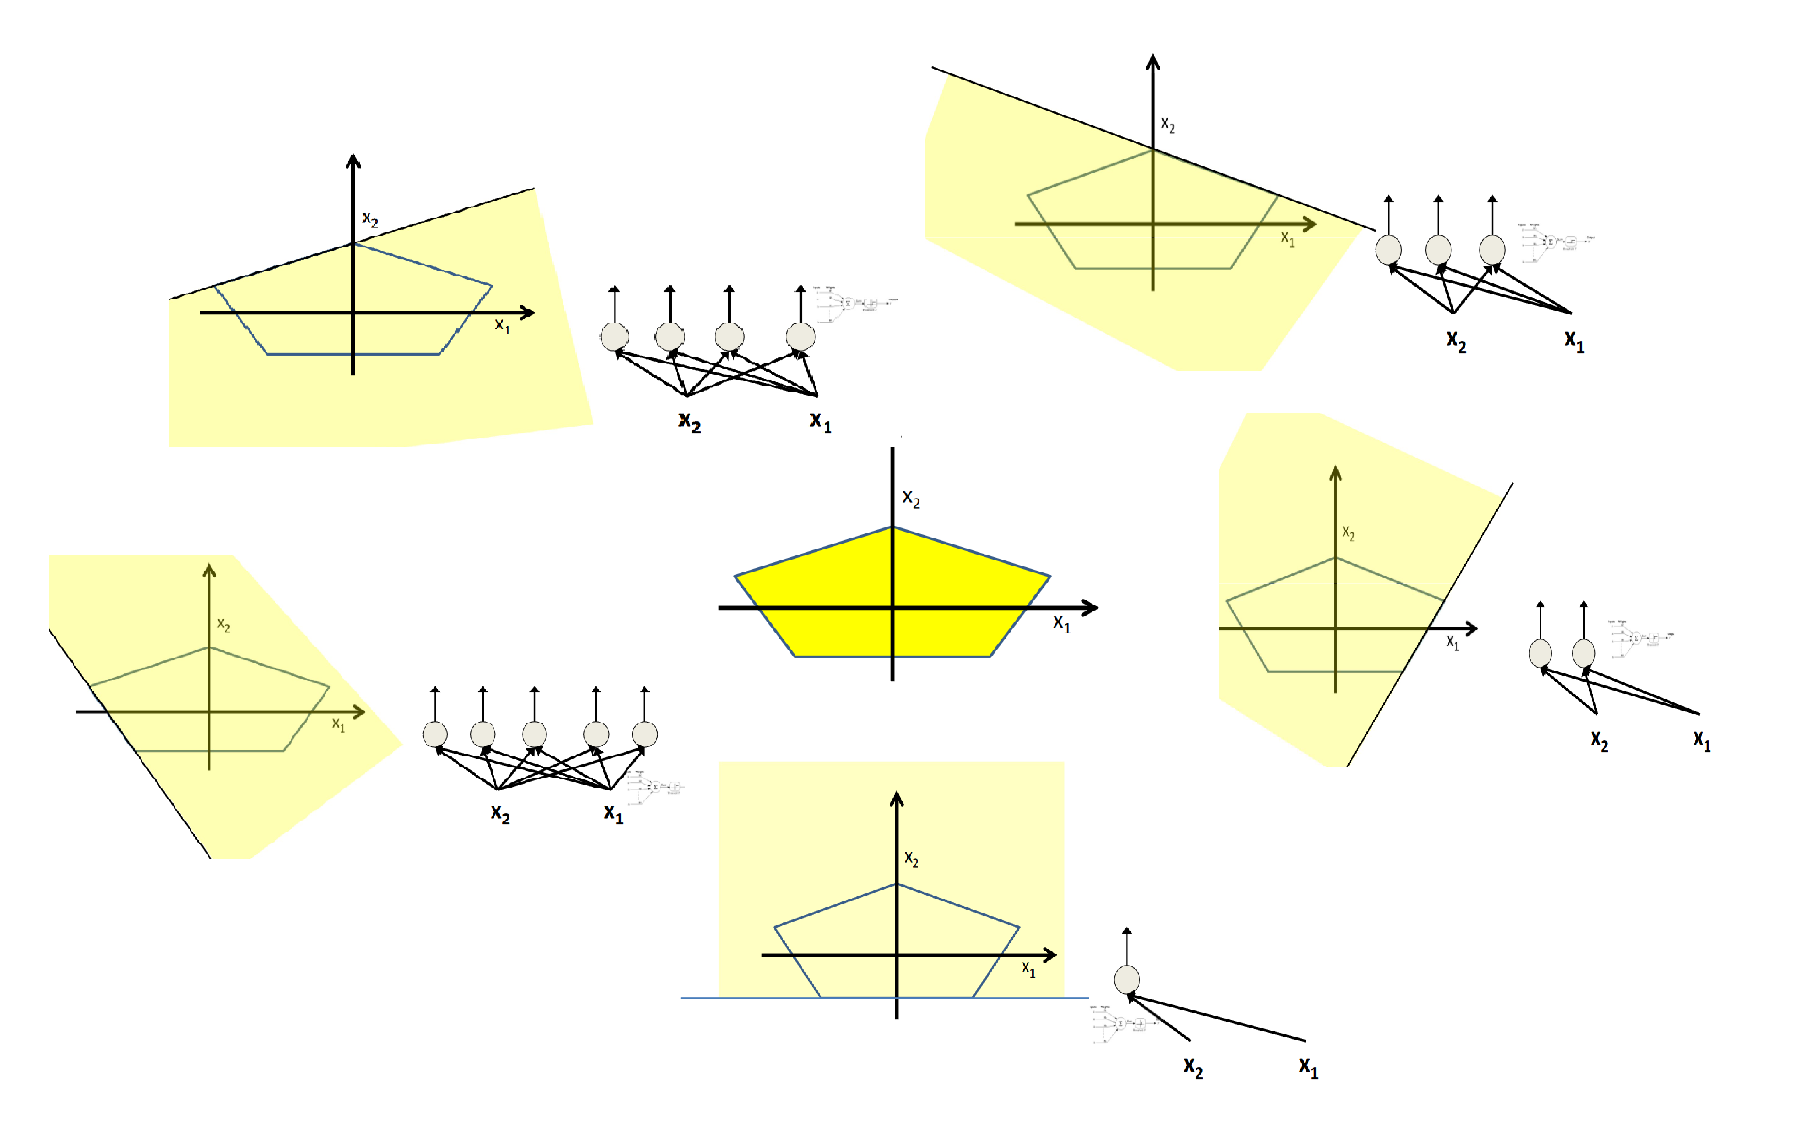
\includegraphics[width=\textwidth]{1_multi_model_perceptron}
\end{figure}

\hfill\break
Given this perceptrons, we can AND them together capture the pentagon decision boundary.

\begin{figure}[H]
	\centering
	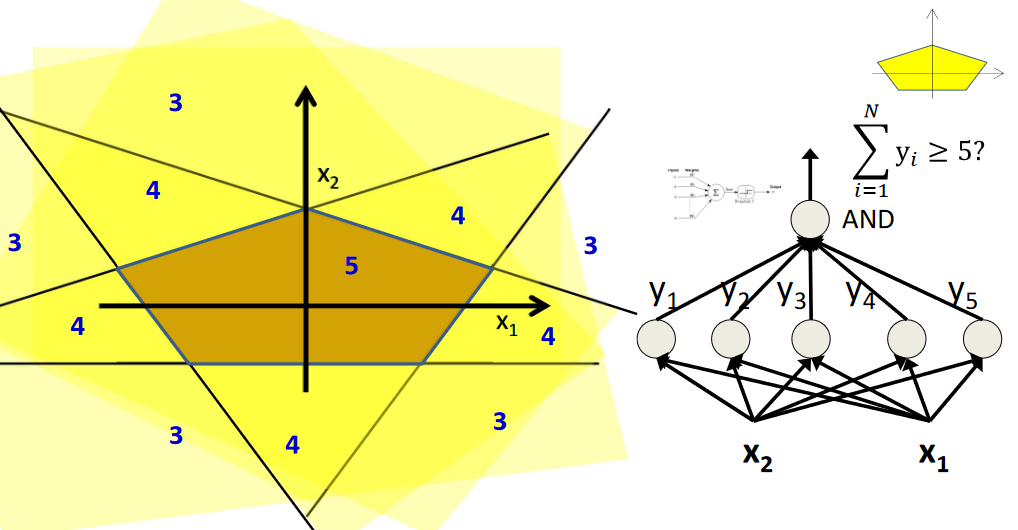
\includegraphics[width=\textwidth]{1_pentagon}
\end{figure}

\hfill\break
This also imply that much more complex boundary condition can be solved as well.

\begin{figure}[H]
	\centering
	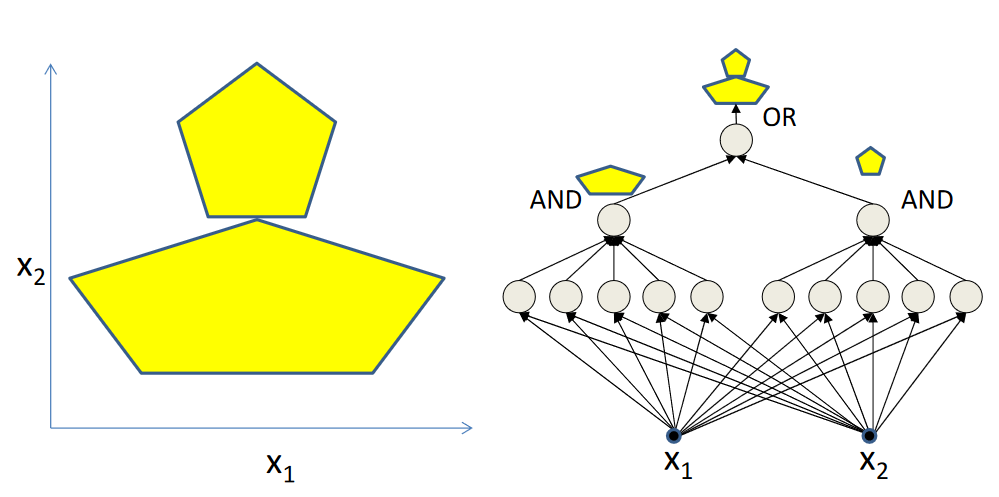
\includegraphics[width=\textwidth]{1_complex}
\end{figure}

\hfill\break
The network will fire if the input is in the yellow area:
\begin{itemize}
	\item "OR" two polygons
	\item This would means that a third layer of perceptron that behaves as "OR" gate is required.
\end{itemize}

\hfill\break
As the multi-layered perceptron is capable to solve complex decision boundaries, it can be used to solve:
\begin{itemize}
	\item Classification problems - finding decision boundaries in high-dimensional space.
	\item For example, the MNIST dataset every image as at least 784 dimensions boundary that need to be solved.
	\item MLP can be considered as universal classifiers as for any decision boundary, we can construct MLP that captures it with arbitrary precision.
\end{itemize}

\subsection{Continuous Valued Outputs}
So far we have covered networks which have Boolean functions where the inputs were Boolean and the output was Boolean. We also discussed functions that took continuous valueed inputs that gave Boolean or categorical output. This section covers the possibility of the networks having real-valued inputs with continuous valued output.

\hfill\break
Consider a simple three units MLP:
\begin{figure}[H]
	\centering
	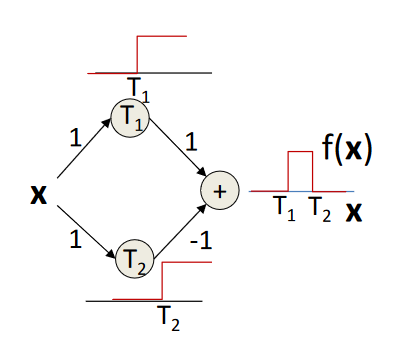
\includegraphics[width=0.5\textwidth]{1_3_unit_mlps}
\end{figure}

\begin{itemize}
	\item The input is a single scalar $\mathbf{x}$.
	\item The first neuron fires, meaning that the output becomes $1$ anytime the input $\mathbf{x}$ exceed the threshold value $T_1$.
	\item The second neuron also fires, meaning that the output becomes $1$ anytime the input $\mathbf{x}$ exceed the threshold value $T_2$.
	\item Their outputs are summed with values $1$ and $-1$ respectively.
	\item As $\mathbf{x}$ goes from large negative value to large positive value, assuming without loss of generality $T_1 < T_2$, eventually it will cross $T_1$ (At this point it has not yet crossed $T_2$).
	\item So at the first perceptron, the output is $1$ while it is still $0$ on the second perceptron.
	\item As we continue to increase $\mathbf{x}$, it will eventually crosses $T_2$ and the output of these 2 neurons will cancel out.
	\item The output of the overall circuit goes back to zero after passing $T_2$.
	\item This network will output $1$ if the input is between $T_1$ and $T_2$, and zero elsewhere.
\end{itemize}

\hfill\break
Suppose that we are given arbirary function as shown below:
\begin{figure}[H]
	\centering
	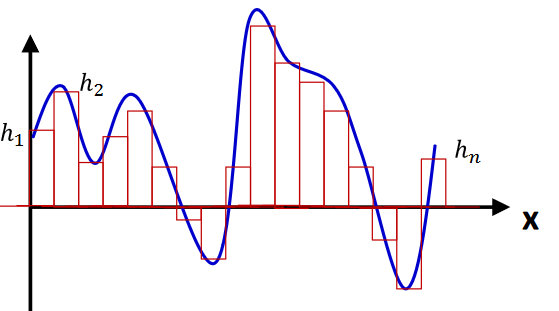
\includegraphics[width=0.5\textwidth]{1_arbitrary_continuous}
\end{figure}

\hfill\break
We can partition the input space into lots of little buckets (similar how ADC works), so that we can have one little subnet for each of the bucket. Then we can scale the outputs by the height of the function average within that range.

\begin{itemize}
	\item An MLP with many units can model an arbirary function over an input.
	\item We can get an arbirary precision by making the individual buckets smaller.
	\item This generalizes to functions of any number of inputs.
\end{itemize}

\subsection{Summary}
\begin{itemize}
	\item MLPs are connectionist computational models.
	\begin{itemize}
		\item Individual perceptrons are computational equivalent of neurons.
		\item The MLP is a layered composition of many perceptrons.
	\end{itemize}
		\item MLPs can model any Booleans function.
	\begin{itemize}
		\item Individual perceptrons can act as Boolean gates.
		\item Networks of perceptrons are Boolean gates.
		\item MLPs are universal Boolean functions.
	\end{itemize}
		\item MLPs can models any decision boundary.
	\begin{itemize}
		\item Individual perceptrons capture linear boundaries.
		\item Complex boundaries can be composed from the linear boundaries.
		\item MLPs can represent arbitrary decision boundaries.
		\item They can be used to classify data.
		\item MLPs are universal classifiers.
	\end{itemize}
\end{itemize}
	\newpage
\section{Chapter 2}

\begin{figure}[H]
	\centering
	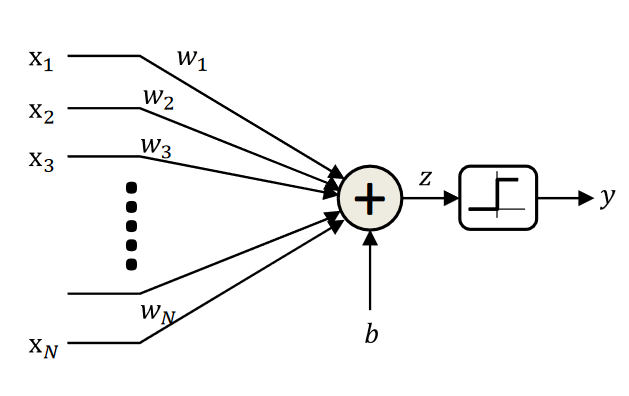
\includegraphics[width=0.5\textwidth]{2_perceptron}
\end{figure}

\hfill\break
Each individual neurons can be represented as a threshold unit.
\begin{itemize}
	\item It fires if the affine function of inputs is positive.
	\item The bias value is the negative of threshold $T$.
\end{itemize} 

\begin{align*}
	z &= \sum_{i}w_ix_i + b \\
	y &= 
\begin{cases} 
	1, & \text{if } z \geq 0 \\
	0, & \text{else }
\end{cases}
\end{align*}

\hfill\break
Once we can represent the neuron in this manner, we can modify the activation threshold function to something different such as:
\begin{itemize}
	\item We define \textbf{activation function} as the function that acts on the weighted combination of inputs and bias.
	 
\end{itemize}
\paragraph{Soft Perceptron (Logistic)}
A squashing function instead of a threshold at the output. This way the output goes rather smooth from $0$ to $1$.
\begin{align*}
	z &= \sum_{i}w_ix_i + b \\
	y &= \frac{1}{1 + \exp (-z)}
\end{align*}

\hfill\break
We can also replace the activation function with other mathematical function such as $\tanh$, $\text{softplus}$ and $\text{rectifier}$.

\subsection{Multi-layer Perceptron}
MLP is a network of perceptrons as the perceptrons of current layer are fed to other perceptrons on the next layer.

\paragraph{Deep Structures}
In any directed graph with input source nodes and output sink nodes, ``depth'' is the length of the longest path from a source to a sink.
\begin{itemize}
	\item A ``source'' node in a directed graph is a node that has only outgoing edges.
	\item A ``sink'' node is a node that has only incoming edges.
\end{itemize}

\hfill\break
This is an example of depth 2 graph.
\begin{figure}[H]
	\centering
	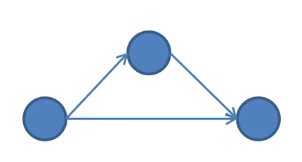
\includegraphics[width=0.4\textwidth]{2_2depth}
\end{figure}

\hfill\break
This is an example of depth 3 graph.
\begin{figure}[H]
	\centering
	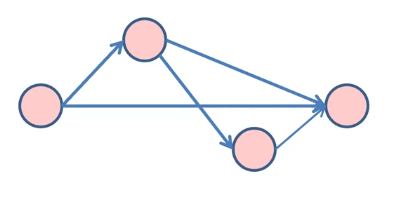
\includegraphics[width=0.4\textwidth]{2_3depth}
\end{figure}

\hfill\break
In multilayer perceptron, a network is considered ``deep'' if the depth of the output neurons is greater than $2$.

\subsection{Layer}
Layer is a set of neurons that are all at the same depth  with respect to the input (sink). This would imply that the ``depth'' of the layer is the depth of the neurons in the layer with respect to the input.

\begin{figure}[H]
	\centering
	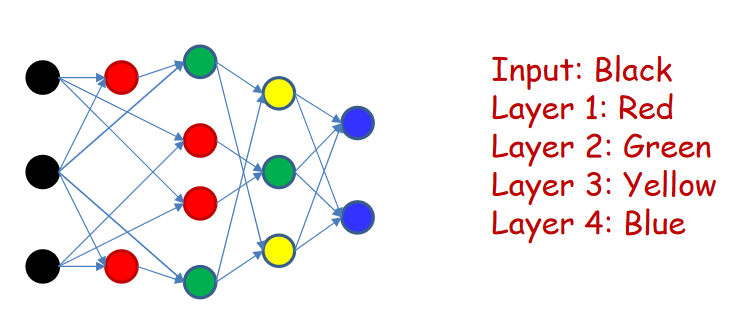
\includegraphics[width=0.75\textwidth]{2_layer}
\end{figure}

\hfill\break
In multi-layered perceptron:
\begin{itemize}
	\item Inputs are real or Boolean stimuli.
	\item Outputs are real or Boolean values.
	\item It can compose both Boolean and real-valued functions.
	\item We can have multiple outputs for a single input.
\end{itemize}

\subsection{MLP as universal Boolean functions.}
We are already aware with perceptron capability as a Boolean gate as it can model any simple binary Boolean gate (OR, AND \& NOT).

\begin{figure}[H]
	\centering
	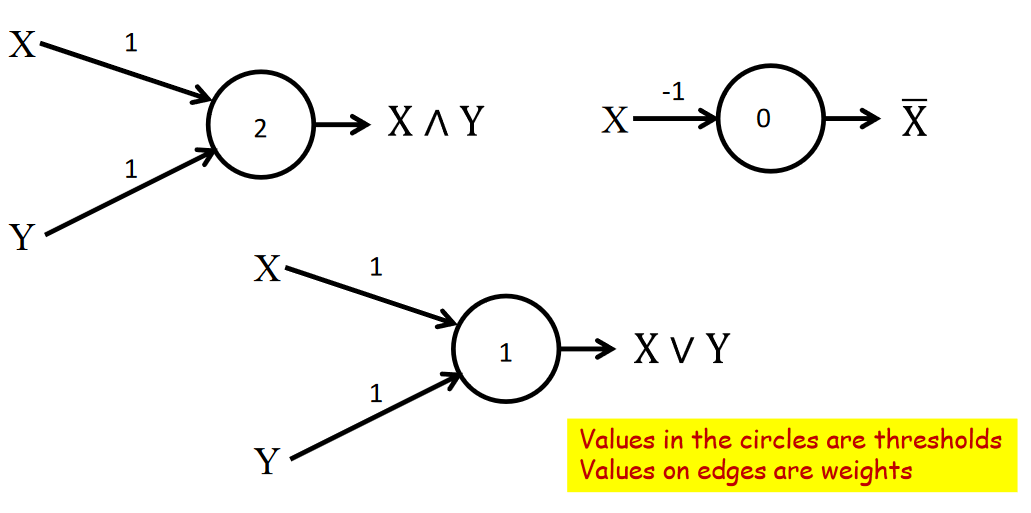
\includegraphics[width=\textwidth]{2_boolean_gate}
\end{figure}

\begin{itemize}
	\item For the AND gate, the boundary condition is $X + Y \geq 2$
	\item For the OR gate, the boundary condition is $X + Y \geq 1$
	\item For the NOT gate, the boundary condition is $-X \geq 0$
\end{itemize}

\hfill\break
It also enables us to compose a much more complex network, for example a universal AND gate where the network is only fired if every input fed to the network is true.

\paragraph{Universal AND Gate}

\begin{figure}[H]
	\centering
	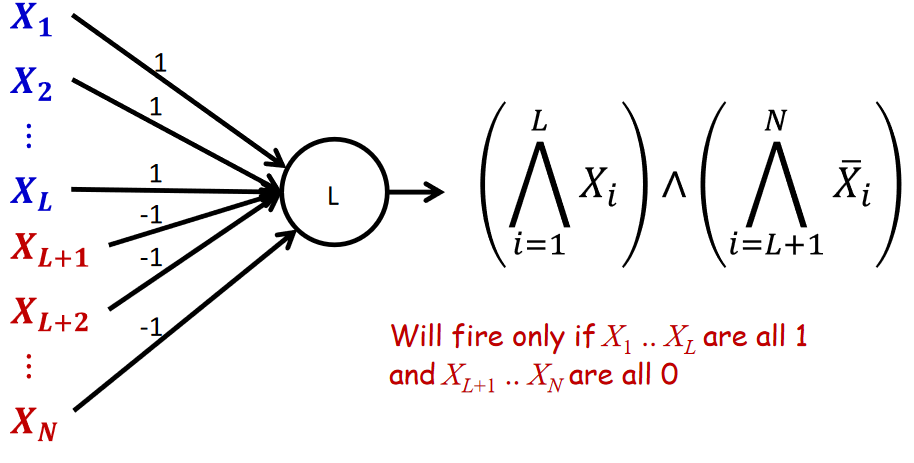
\includegraphics[width=0.5\textwidth]{2_universal_and}
\end{figure}

Suppose that $X_1,X_2,...,X_L$ has weight value of $1$ and $X_{L+1},X_{L+2},...,X_N$ has weight value of $-1$, the condition for the perceptron to fire has to be:
\begin{align}
	(X_1+X_2+...+X_L) - (X_{L+1},X_{L+2},...,X_N) \geq L
\end{align}

\paragraph{Universal OR Gate}

\begin{figure}[H]
	\centering
	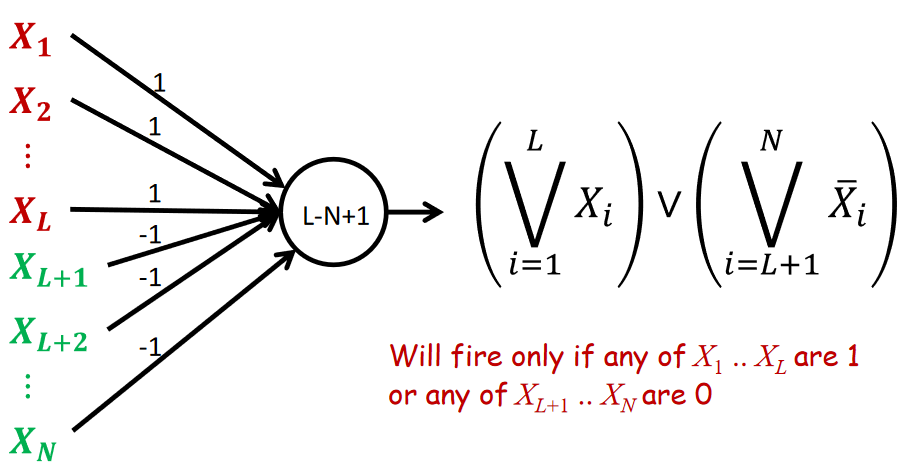
\includegraphics[width=0.5\textwidth]{2_universal_or}
\end{figure}

Suppose that $X_1,X_2,...,X_L$ has weight value of $1$ and $X_{L+1},X_{L+2},...,X_N$ has weight value of $-1$, the condition for the perceptron to fire has to be if any value of the first set is $1$ or any value from the second set is $0$:
\begin{align}
	(X_1+X_2+...+X_L) - (X_{L+1},X_{L+2},...,X_N) \geq L - N + 1
\end{align}

\paragraph{Generalized Majority Gate}

\begin{figure}[H]
	\centering
	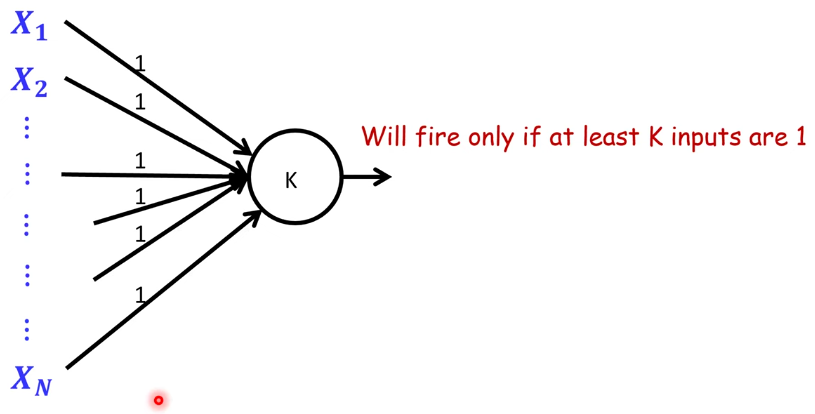
\includegraphics[width=0.5\textwidth]{2_majority_gate}
\end{figure}

\hfill\break
Due to perceptrons being able to model Boolean functions, they able to model complex things that are made of Boolean functions. This also means that for any odd Boolean function, wee can construct a multi-layerr perceptron that can compute this Boolean function. This is what is meant by MLPs being a universal Boolean functions. For any Boolean functions, regardless of their complexity, we can compose an MLP that will compute said function. This lead to a new question, how many layers will they need to be sufficient at modeling said Boolean function? What is the smallest number of layers will be required?


\hfill\break
Any Booleans function can be represented by a truth table. For example:


\begin{table}[H]
	\centering
	\begin{tabular}{|c|c|c|c|c|c|}
			\hline
			$X_1$    & $X_2$     & $X_3$    & $X_4$    & $X_5$    & $Y$   \\
			\hline
			0        & 0        & 1        & 1        & 0        & 1     \\
			0        & 1        & 0        & 1        & 1        & 1     \\
			0        & 1        & 1        & 0        & 0        & 1     \\
			1        & 0        & 0        & 0        & 1        & 1     \\
			1        & 0        & 1        & 1        & 1        & 1     \\
			1        & 1        & 0        & 0        & 1        & 1     \\
			\hline
	\end{tabular}
\end{table}

\hfill\break
In order to get a Boolean function that represent this table, we only have to list the portion of the table that corresponds to the output 1. We can write it as disjunctive normal formula for this table. 

\begin{align}
	Y = \bar{X_1}\bar{X_2}X_3X_4\bar{X_5} + \bar{X_1}X_2\bar{X_3}X_4X_5 + \bar{X_1}X_2X_3\bar{X_4}\bar{X_5} +\\ X_1\bar{X_2}\bar{X_3}\bar{X_4}X_5 + X_1\bar{X_2}X_3X_4X_5 + X_1X_2\bar{X_3}\bar{X_4}X_5
\end{align}

\hfill\break
Once we have obtained the Boolean function in this manner, we can create an MLP where each of the perceptron is an Universal AND gate. These perceptrons is then combined as Universal OR gate.


\begin{figure}[H]
	\centering
	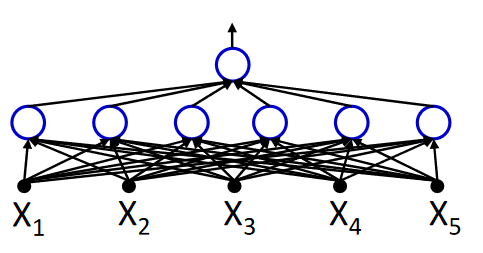
\includegraphics[width=0.5\textwidth]{2_truth_table}
\end{figure}

\hfill\break
This would means that MLP with 1 layer is sufficient enough to model any Boolean Function. This lead to a new question, what is the largest number of perceptrons required in the single hidden layer for an N-input-variable function?

\subsection{Karnaugh Map}
Boolean function can be reduced using Karnaugh Map. It represent a truth table as a grid. Adjacent boxes can be ``grouped'' to reduce the DNF formula for the table.

%\begin{figure}[H]
%\centering
%\begin{Karnaugh}{$v_w$}{$x_y$}
%	\content{0,0,0,0,0,0,0,0,0,0,0,0,0,0,0,0}
%	\implicant{0}{2}{red}
%	\implicant{5}{15}{purple}
%	\implicanttopbottom[3pt]{1}{10}{blue}
%	\implicantcorners[2pt]{orange}
%	\implicantside{4}{14}{green}
%\end{Karnaugh}
%\end{figure}

\begin{figure}[H]
	\centering
	\begin{Karnaugh}{$WX$}{$YZ$}
		\content{1,0,1,0,1,1,0,0,1,0,1,0,1,0,0,0}
		\implicant{4}{5}{red}
		\implicant{0}{8}{blue}
		\implicanttopbottom[3pt]{2}{10}{green}
	\end{Karnaugh}
\end{figure}

\hfill\break
We can group these 3 neighbours together:

\begin{align}
	O = \bar{Y}\bar{Z} + \bar{W}X\bar{Y} + \bar{X}Y\bar{Z}
\end{align}

\begin{itemize}
	\item Regardless value of $W$ and $X$, $Y$ and $Z$ is always $0$.
	\item The function going to fire when $W$ is always $0$ while $X$ can be anything, while $Y$ has to always be $0$.
	\item The other condition for it to fire is when $Y$ is always $1$ while $Z$ is always $0$ and $X$ is always $0$.
\end{itemize}


\hfill\break
Although there are 8 conditions when the network will fire, only 3 perceptions is needed to construct the MLP. The general idea is, when we want to construct the DNF formula, we want to construct it with thee minimum number of clauses.

\begin{figure}[H]
	\centering
	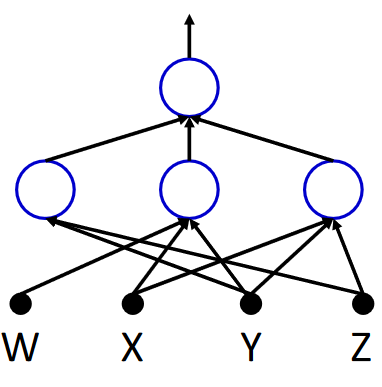
\includegraphics[width=0.5\textwidth]{2_reduced_dnf}
\end{figure}

\hfill\break
On irreducible DNF, the size of required perceptrons in the hidden layer can get exponentially large ($2^{n-1}$).

\begin{figure}[H]
	\centering
	\begin{Karnaugh}{$WX$}{$YZ$}
		\content{1,0,0,1,0,1,1,0,0,1,1,0,1,0,0,1}
	\end{Karnaugh}
\end{figure}

\hfill\break
While the DNF cannot be reduced, this type of Boolean function can still be generalized. Is it possible to reduce the number of units if we use multiple hidden layers?

This checkered pattern is a form of XOR Boolean function which become TRUE only if:
\begin{itemize}
	\item 1 flag is FALSE while the rest of the flags is TRUE.
	\item 1 flag is TRUE while the rest of the flags is FALSE.
\end{itemize}

\begin{align}
	O = W \oplus X \oplus Y \oplus Z
\end{align}

\hfill\break
Since we need 1 hidden layer consisting of 2 perceptrons to construct XOR gate:

\begin{figure}[H]
	\centering
	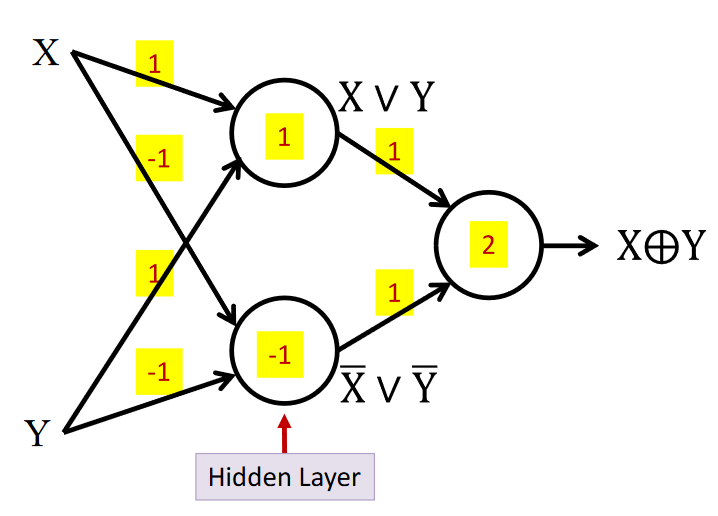
\includegraphics[width=0.5\textwidth]{2_xor}
\end{figure}

\hfill\break
We can cascade the XOR gates to construct the solution for the MLP.

\begin{figure}[H]
	\centering
	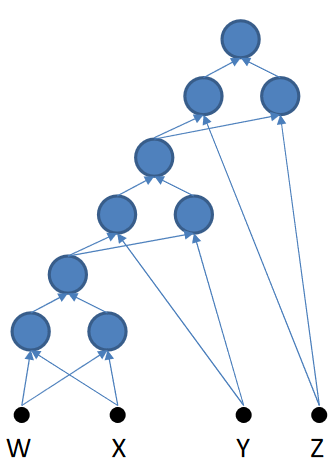
\includegraphics[width=0.5\textwidth]{2_xor_cascade}
\end{figure}

\hfill\break
For cascading XOR gates with 4 parameter, 9 perceptrons would be required to construct the Boolean function MLP. The solution of the cascading XOR gates would be $3\times (N-1)$ number of perceptrons. 

These can be arranged in only $2\log_2(N)$ layers. Suppose that wee have $X_1, X_2, ..., X_N$ number of perception. We can keep pairing terms such as:

\begin{align}
	O &= X_1 \oplus X_2 \oplus X_3 \oplus X_4 \oplus X_5 \oplus X_6 \oplus X_7 \oplus X_8\\
	O &= ((X_1 \oplus X_2) \oplus (X_3 \oplus X_4)) \oplus ((X_5 \oplus X_6) \oplus (X_7 \oplus X_8))
\end{align}

\begin{figure}[H]
	\centering
	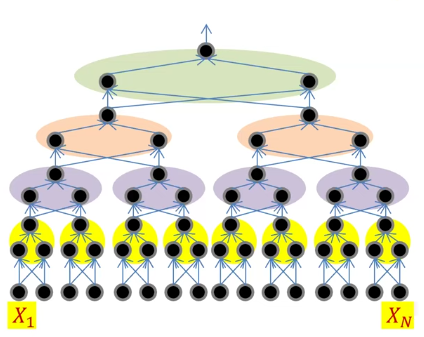
\includegraphics[width=0.75\textwidth]{2_multi_layer_xor}
\end{figure}

\subsection{Implementation of MLP on K-layer.}
Using only K-hidden layers will require $2^{CN}$ neurons in the K-th layer, where

\begin{align}
	C = 2^{-\frac{K-1}{2}}
\end{align}

\begin{figure}[H]
	\centering
	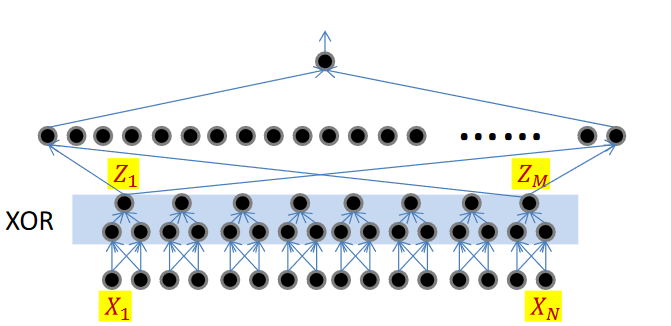
\includegraphics[width=0.75\textwidth]{2_k_layer_xor}
\end{figure}

\hfill\break
Going through the layer until the K-th layer, we keep reducing the number of neutrons by factor of $2$. However, we still have to XOR whatever number of neutrons left on the K-th layer, exponentially increasing the number of neutrons.

\begin{itemize}
	\item Because the output is the XOR for all the $\frac{N}{2^{\frac{K-1}{2}}}$ values output by the K-1-th hidden layer.
	\item In other word, reducing the numbers of layers below the minimum will result in an exponentially sized network to express the function fully.
	\item A network with fewer than minimum required number of neutrons cannot model the function.
\end{itemize}

\subsection{Network Parameters.}
The actual number of parameters in a network is the number of connections. For example, for a network with 1 hidden layer consisting of 5 neutrons, the number of parameters in a network is 30.

\begin{figure}[H]
	\centering
	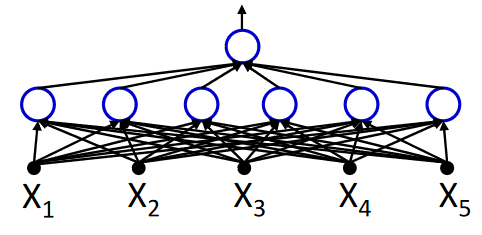
\includegraphics[width=0.75\textwidth]{2_1_layer_mlp}
\end{figure}

This is the number that really matters in software or hardware implementation of the neural networks. Networks that require an exponential number of neurons will require an exponential number of weights.

\subsection{Composing complicated ``decision'' boundary.}
Once we can computes a linear boundary, we can compose more complex decision boundary as shown below.

\begin{figure}[H]
	\centering
	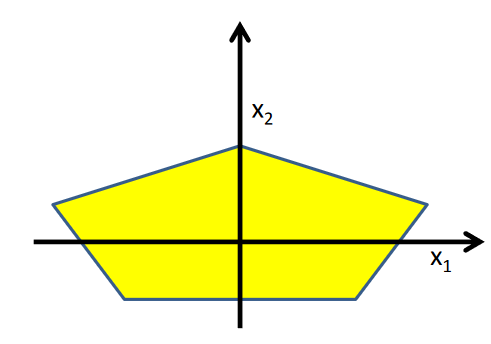
\includegraphics[width=0.5\textwidth]{2_penta_boundary}
\end{figure}

\hfill\break
Recall that should we have pentagonal boundary, that would means that we have boundaries for each sides of the pentagon and the network will fire if the input value exceeds the boundary threshold value. One thing to notice that, only within the pentagon are all five perceptrons going to output $1$. This would imply that the network will fire if \textbf{sum of all of the output} exceeds the \textbf{sum of the threshold boundary value}.

\begin{figure}[H]
	\centering
	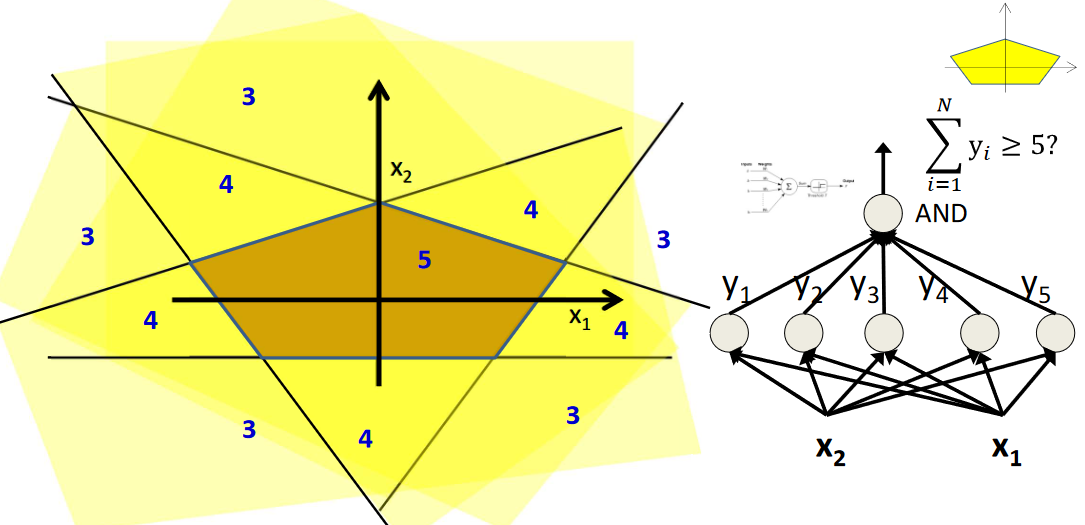
\includegraphics[width=\textwidth]{2_sum_output}
\end{figure}

And if there is more than one closed boundaries, we have to OR them together to get the complex decision boundary. This would means that a third layer would be required.

\begin{figure}[H]
	\centering
	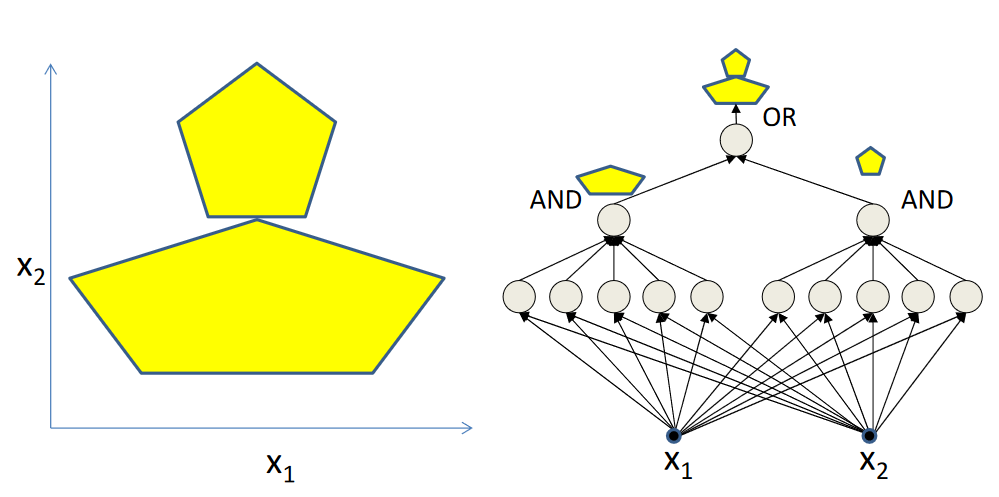
\includegraphics[width=\textwidth]{1_complex}
\end{figure}

The question is, is it possible to compose these decision boundaries with only one hidden layer?

\hfill\break
\textbf{Case: Square boundary}
\\\\
The sum of the output of the inner boundary is 4. Instead of having output layer of AND-ing all of the output of the previous layer perceptron, we just set the threshold value to be the sum of the threshold value of the individual perceptron. The last output neuron is performing SUM instead of AND.

\begin{figure}[H]
	\centering
	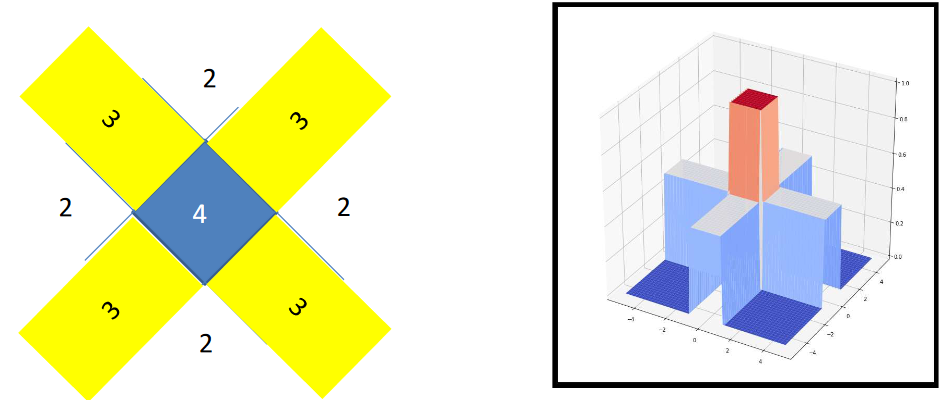
\includegraphics[width=\textwidth]{2_square_boundary}
\end{figure}

\hfill\break
\textbf{Case: Pentagon boundary}

\begin{figure}[h]
	\centering
	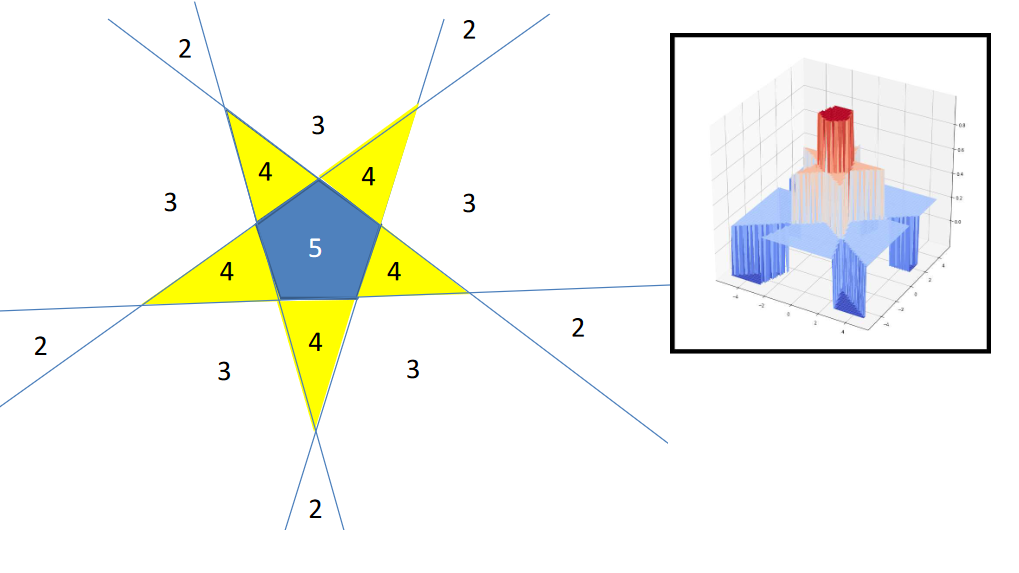
\includegraphics[width=\textwidth]{2_pentagon_boundary}
\end{figure}

\hfill\break
\textbf{Case: Hexagon boundary}

\begin{figure}[H]
	\centering
	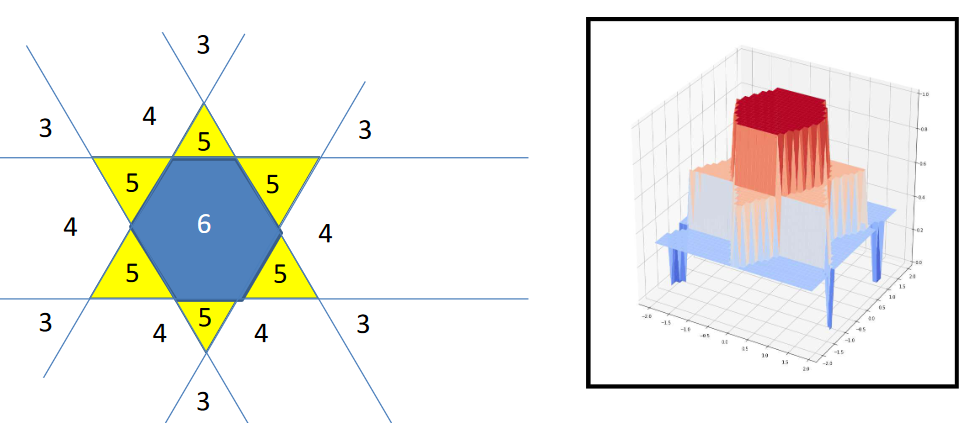
\includegraphics[width=\textwidth]{2_hexagon_boundary}
\end{figure}

\hfill\break
What if we want to compose composite decision boundary with single hidden layer?

\begin{figure}[H]
	\centering
	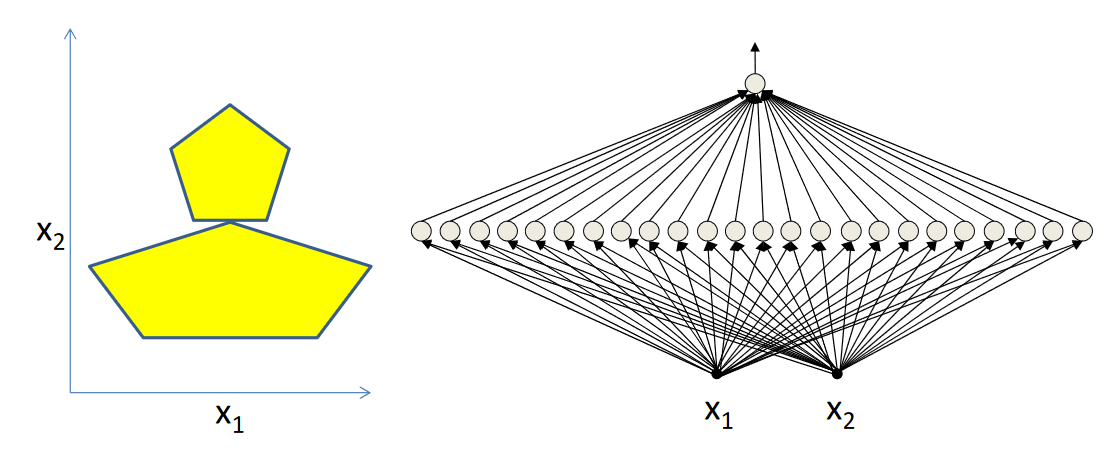
\includegraphics[width=\textwidth]{2_composite_boundary}
\end{figure}

\hfill\linebreak
If we could just somehow finagle these boundaries, it would not be possible because some of the sides of the lower pentagon will intercept with some of the edges of the upper pentagon. So any threshold that can capture lower pentagon will accidentally capture the upper pentagon region that is outside of the region of the lower pentagon.

Consider a square polygon. We would need a network with four neuron in a hidden layer to be able to describe the decision boundary. The threshold value on the side area of the polygon would be 3 and the rest of the area will have threshold value of 2. The same principle will apply to higher dimension polygon where the threshold value would be $s$, $s-1$, $s-2$ $...$ .

We can observe that the first outer layer that is adjacent with the decision boundary would have $s-1$ threshold value. Another observation that could be noticed is that the sum of the area that is outside the decision boundary will always bigger than the sum inside poligon.

\hfill\linebreak
\textbf{Case: Pentagon}

\begin{align*}
	\text{Inner threshold value} &= 5 \\
	\text{Sum of the threshold value of the first outer layer} &= 4 \times 5 \\
	&= 20 \\
	\text{Sum of the threshold value of the second outer layer} &= 3 \times 5 \\
	&= 15 \\
	\text{Sum of the threshold value of the last outer layer} &= 2 \times 5 \\
	&= 10 \\
\end{align*}

\hfill\break
Another observation that could be made is that as the number of the decision boundary increases, the size of the first outer layer will be decreasing. Looking back at the possibility of creating single layer MLP for composite boundary, say if we want to compose a single hidden layer MLP for these outer regions, it would be possible only if the region is really small and does not overlap with the first outer region of another boundary. That being said, constructing MLP for composite boundaries would be possible if these regions are so small that it would not overlap with each other.

\hfill\break
Since for any polygons, the size of the first outer layer will be smaller as the number of sides / decision boundary increases, this would means a circle would have the smallest area of first outer layer since the number of edges $\rightarrow\infty$. Increasing the number of sides will reduces the area outside the polygon that have $\frac{N}{2}<\sum_{i}{y_i}<N$.

\hfill\break
Hypothetically speaking, this would means for a single layer MLP for decision boundary of circle:
\begin{itemize}
	\item The number of neurons will become infinitely large.
	\item Sum of N inside the circle, $\frac{N}{2}$ outside almost everywhere.
\end{itemize}

\begin{figure}[H]
	\centering
	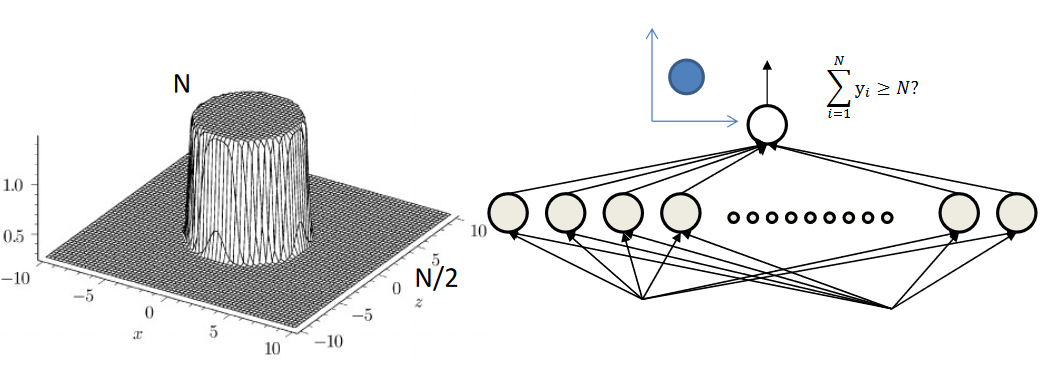
\includegraphics[width=\textwidth]{2_circle_mlp}
\end{figure}

Based on the MLP constructed, if we sum all of these outputs and use a threshold:

\begin{align}
	\sum^N_{i=1}\mathbf{y}_i - \frac{N}{2} \geq 0
\end{align}

\hfill\break
A decision boundary for a perfect circle can be obtained. We also can take a 2 different circle subnets which compose of circles in two different position and still use the same threshold value on the output perceptron. This is because the ``sum'' of two circles of the individual subnets is exactly $\frac{N}{2}$ inside either circle and almost $0$ everywhere outside of the circles.

\begin{figure}[H]
	\centering
	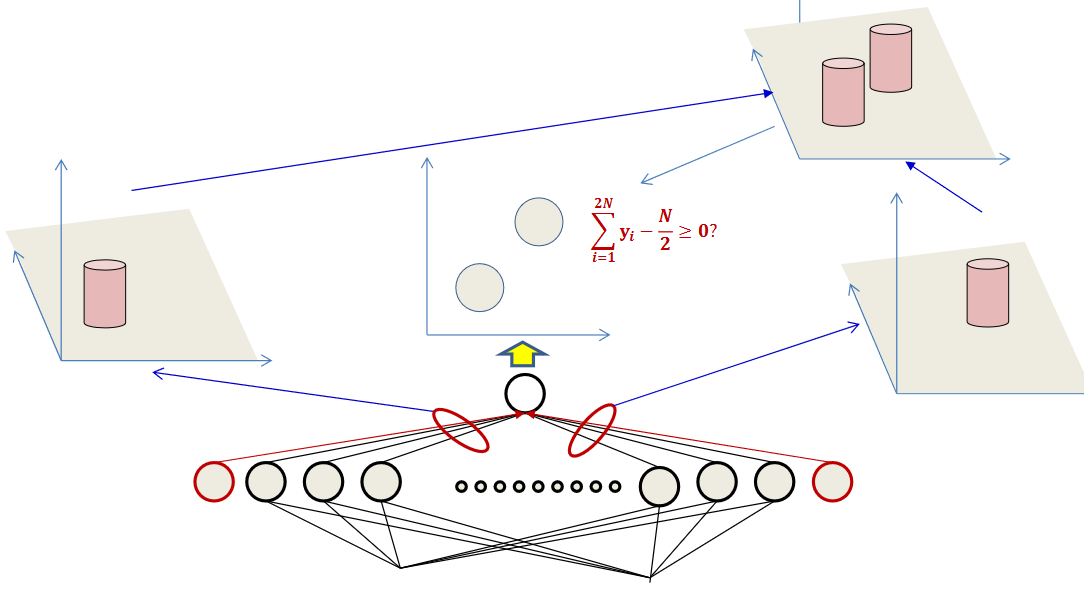
\includegraphics[width=\textwidth]{2_multiple_circles}
\end{figure}

\hfill\break
This would also means that it is possible to use subnets of circle decision boundary to compose any arbitrary figure. We just have have to fill in the composite shapes with enough circle decision boundary. An accurate approximation could be achieved with greater number of smaller circles. This demonstrate the capabilities of one hidden layer MLP being able to model any classification boundary with enough number of neurons.

\begin{figure}[H]
	\centering
	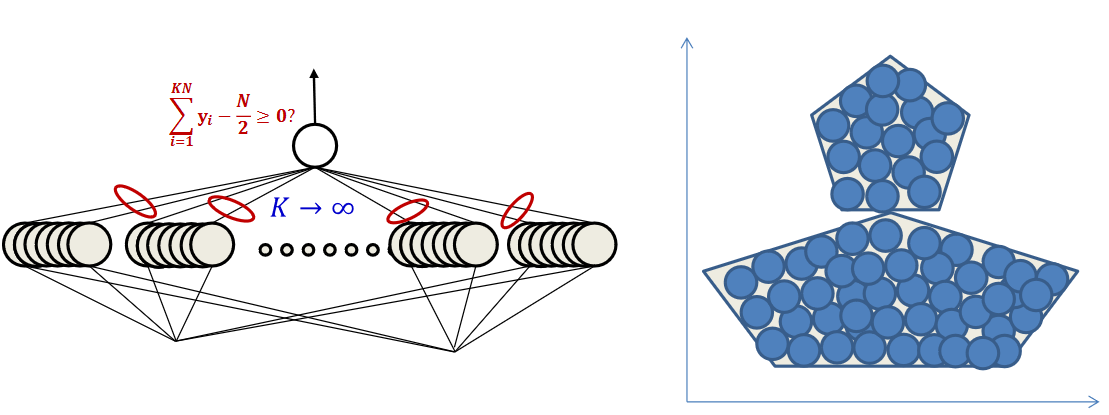
\includegraphics[width=\textwidth]{2_circle_mlp_composite}
\end{figure}

\subsection{Performance comparison between deep network and single layer network.}
 
 \begin{figure}[H]
 	\centering
 	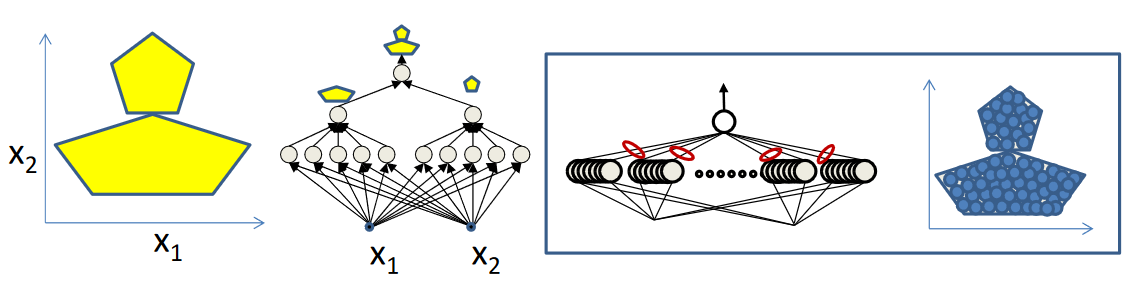
\includegraphics[width=\textwidth]{2_deep_vs_one}
 \end{figure}
 
Deep networks require far fewer neutrons to achieve the same result. Depending on the compleexity of the decision boundary, a naive one-hidden-layer neural network will require infinite hidden neurons. For example, consider an image below, a single layer MLP would require infinite amount of neurons as sum of subset of the circles that is going to be filled into the yellow region.

 \begin{figure}[H]
	\centering
	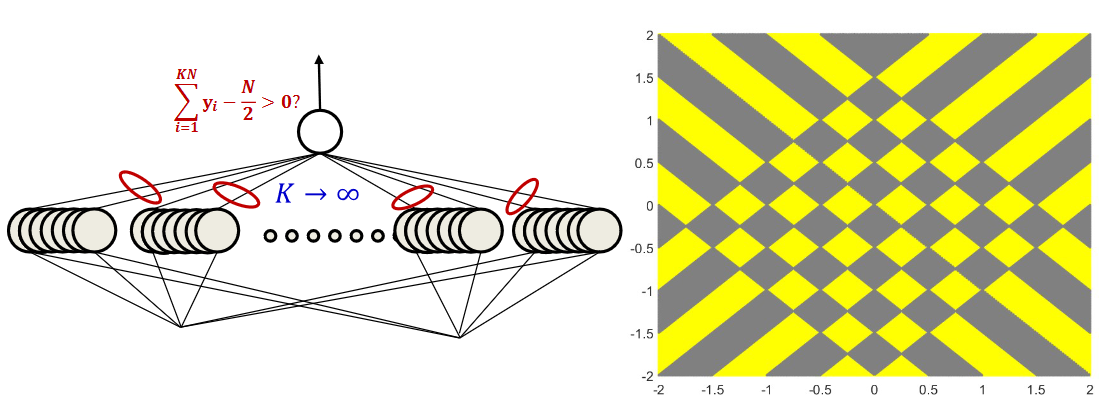
\includegraphics[width=\textwidth]{2_infinite}
\end{figure}

\hfill\break
Howerver, if observed carefully, this image contains 16 lines and 40 segments forming the yellow regions. This would means that we can compose a 2 hidden layer MLP  where every individual neurons on the same layer are XOR-ed together such that

\begin{itemize}
	\item 16 neurons on the first hidden layer.
	\item 40 neurons on the second hidden layer.
	\item 1 neurons on the output layer.
\end{itemize}

 \begin{figure}[H]
	\centering
	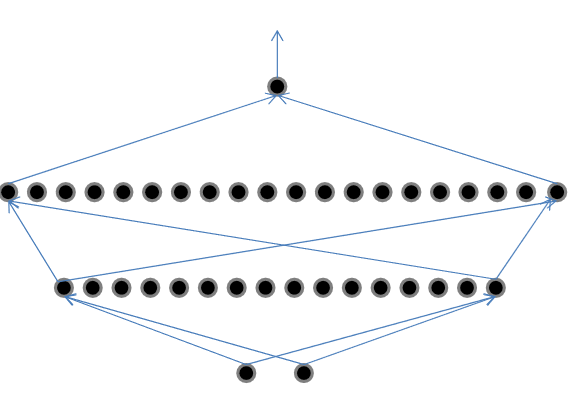
\includegraphics[width=0.5\textwidth]{2_2_layer_mlp}
\end{figure}






























\end{document}